\documentclass[12pt,a4paper]{report}
\usepackage[utf8]{inputenc}
\usepackage{amsmath}
\usepackage{amsfonts}
\usepackage{amssymb}
\usepackage{graphicx}

\title{Relatório 1  \\
	Projeto em Eletrônica I - EEL7801 \\ \vfill
	\normalsize{Universidade Federal de Santa Catarina - UFSC \\
		Professora: Daniela Ota Hisayasu Suzuki}
	\author{
		{Luiz Augusto Frazatto Fernandes: \it{17202752}} \\
		{Leonardo José Held: \it{17203984}}
	}
}
\date{6 de Junho de 2019}
\begin{document}
	\maketitle
	\setcounter{chapter}{0}
	\chapter{Amplificadores e teste}
	\section{Amplificador - Emissor}
		\paragraph{} Utilizando o CI LM386, fez-se um amplificador do sinal sonoro. O circuito fora descrito no Relatóio 1.
	\subsection{Ganhos do sinal}
	\section{Filtro amplificador - Receptor}
		\paragraph{} A fim de se evitar que fossem geradas tensões acima de $5V$ (o Datasheet do MCU recomenda tensões limites de $(5+0.3)V$), colocou-se um diodo zener na saída do circuito, dessa forma limitando o {\it output}. Além disso, caso fosse necessária uma tensão limite de $3.3V$, pode-se colocar um divisor de tensão na saída do regulador.
		
		A resistência mínima a ser colocada em série com o diodo é dado da seguinte maneira:
		
		Dados do diodo:
		\begin{itemize}
			\item[1.] Potência: $P_Z = 1W$;
			\item[2.] Tensão: $V_Z = 5.1V$;
		\end{itemize}
		
		Para a obtenção do valor mínimo de resistência que deve ser adicionado em série com o diodo:
		
		\begin{center}
			\begin{gather}
				V_{max} = 12V\\
				V_Z = 5.1V\\
				I_{Zmax} = \frac{V_Z}{P_Z} = 200mA\\
				R_{min} = \frac{V_{max} - V_Z}{I_{max}} = 34.5\Omega\\
			\end{gather}
		\end{center}
		
		A fim de se garantir a integridade do sinal, mas de ainda termos uma 
		
		Houve, além disso, outra mudança importante no circuito: a fim de se evitar que uma corrente insuficiente seja fornecida para o MCU ou a fim de se preservar a integridade do sinal analógico obtido, fez-se um seguidor de tensão, para que esse fosse desacoplado do sinal original. Para tal mudança, optamos pela troca do chip {\it LM741} pelo chip {\it LM324}.
		
		\begin{figure}[h]
			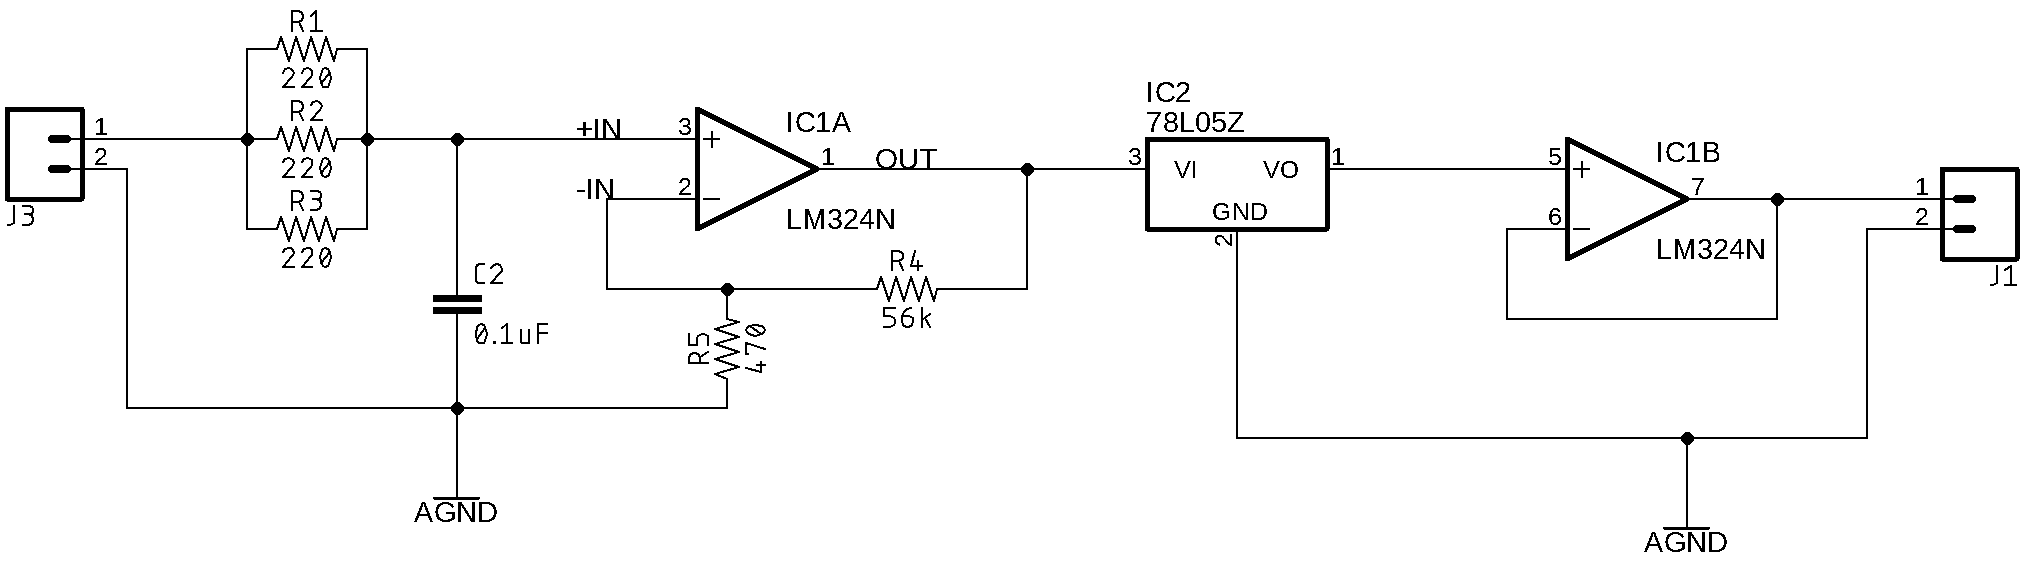
\includegraphics[width=\linewidth]{test.png}
			\caption{Filtro passa baixa amplificador. (Obs.: o CI foi alimentado com $V_s = 12V$ e $GND$)}
			\label{fig:filter}
		\end{figure}
			
	\chapter{Implementação Digital}
	
	\section{Lorem}
	\subsection{title}
	
	\chapter{Implementação Algorítimica}
	
\end{document}